\documentclass[a4paper,11pt,german,notitlepage]{report}
\usepackage{xcolor}
\usepackage{tabularx}
\usepackage{dclecture}
\usepackage{qrcode}
\usepackage{awesomebox}
\usepackage{circuitikz}
\usepackage[style=german, german=swiss]{csquotes}
\def\farbe{darkgray} %Hier Farbe definieren
\addbibresource{refs.bib}

\ctikzset{
    logic ports=ieee,
    logic ports/scale=0.8,
    logic ports/fill=lightgray
}

\usetikzlibrary{arrows,shapes.gates.logic.US,shapes.gates.logic.IEC,calc,positioning}

\graphicspath{{img/}}

% Extract Exercises

%\usepackage[active, generate=trigonometry_exercises, extract-env={ex}]{extract}
%\begin{extract}
%\usepackage{xcolor}
%\def\farbe{teal}
%\usepackage{dcexercisesnogrid}
%\exercisetrue
%\end{extract}


%%% Fancy Header and Footer
\renewcommand{\headrule}{\vbox to 0pt{\hbox to\headwidth{\color{\farbe}\rule{\headwidth}{1pt}}\vss}}
\pagestyle{fancy} %eigener Seitenstil
\fancyhf{} %alle Kopf- und Fu§zeilenfelder bereinigen
\fancyhead[C]{Informatik - Gymnasium 1. Klasse - Algorithmen Projekt - BVB Routenplanung} %Kopfzeile mitte
%\fancyhead[R]{\includegraphics[width=0.2cm]{x.png}}

\fancyfoot[C]{\thepage}

%\rfoot{\setlength{\unitlength}{1mm}
%\begin{picture}(0,0)
%\put(5,0){\includegraphics{pic\thepage.ps}}
%\end{picture}}


\parskip=.1cm
\parindent=0cm
\linespread{1.5}



\begin{document}

\section*{Beschreibung}
In diesem Projekt modellieren Sie einen Ausschnitt des BVB/BLT-Netzes als gewichteten Graphen und entwickeln darauf Suchalgorithmen.
Die Gewichte der Kanten entsprechen Fahrzeiten in Minuten zwischen zwei benachbarten Haltestellen.
\begin{figure}[h!]
    \centering
    
\includegraphics[height=3cm]{logo.png}  
\end{figure}
Ziel ist es, für gegebene Start- und Zielhaltestellen gute und nachvollziehbare Routen zu berechnen.

Der Ausschnitt kann als Graph wie unten dargestellt verstanden werden:
\begin{figure}[h!]
    \centering
    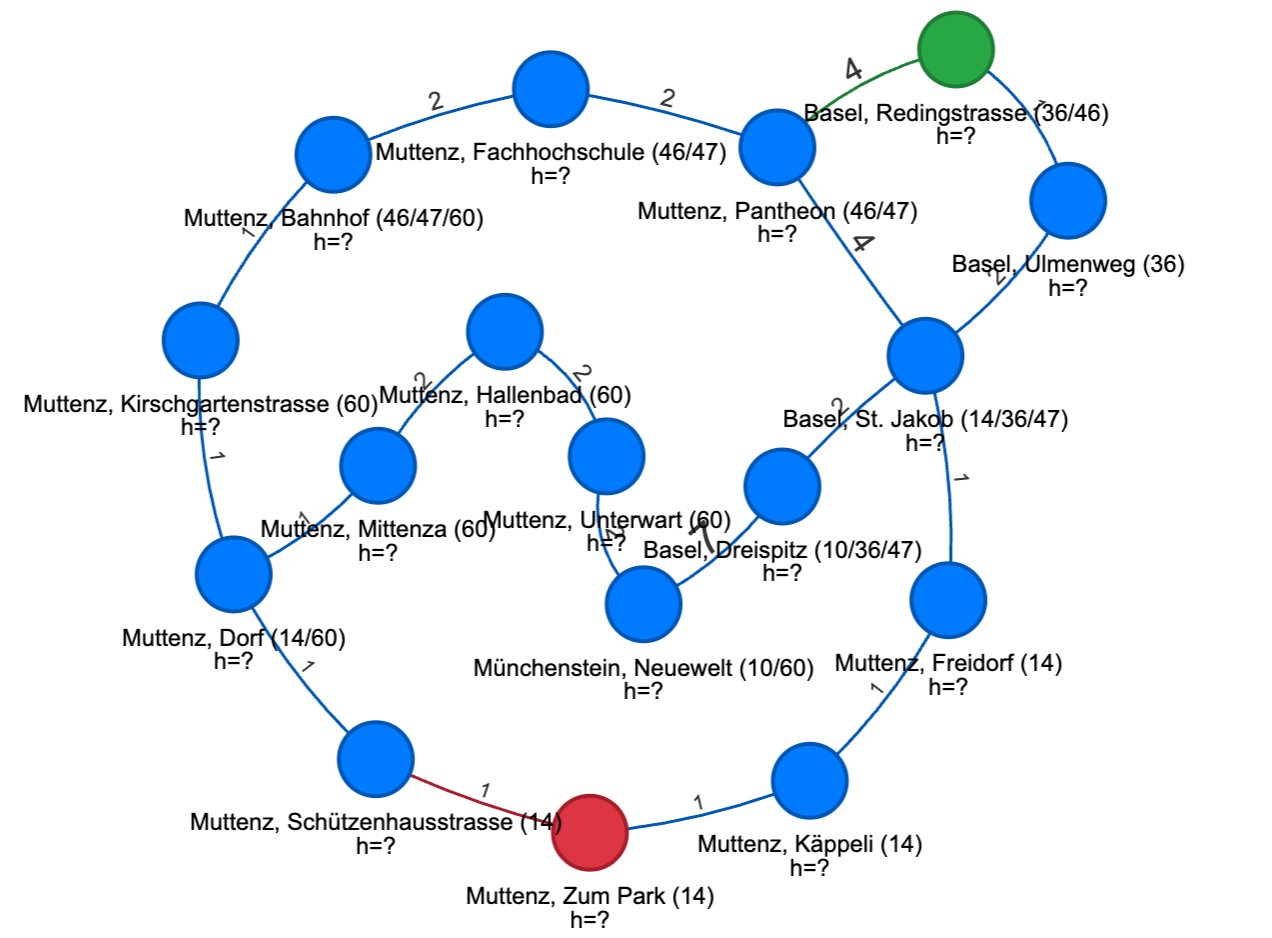
\includegraphics[width=10cm]{netz.png}    
    \caption{Netzausschnitt der BVB. Was wäre hier wohl der schnellste Weg von der Redigerstrasse zur Station zum Park?}
\end{figure}

Als Datengrundlage verwenden Sie den Netzausschnitt, welcher in der Datei \\ \texttt{bvb\_muttenz.json} strukturiert abgelegt ist.

\section*{Zusatzinformationen}
\begin{description}
    \item[Zu erwartender Input:] Start- und Zielhaltestelle aus dem gegebenen Graphen.
    \item[Zu erwartender Output:] Eine Route als Haltestellenfolge, die Gesamtreisezeit und optional die Anzahl untersuchter Zustände.
    \item[Korrektheit:] Eine Route gilt als korrekt, wenn alle aufeinanderfolgenden Haltestellen durch eine Kante verbunden sind.
    \item[Optimalität:] Eine Route gilt als optimal, wenn keine andere Route mit geringerer Gesamtzeit existiert.
\end{description}


\section*{Aufgabe}
Hier werden zusätzliche Aufgaben beschrieben, welche spezifisch für Ihr Projekt sind.
Die Aufgaben sind in zwei Gruppen unterzeilt: Pflichtaufgaben und optionale Aufgaben.
Die Pflichtaufgaben sollen am Ende des Projektes beantwortet sein. Die optionalen
Aufgaben dienen dazu, sich weiter im Thema zu vertiefen. Diese Aufgaben sind Vor-
schläge. Sie dürfen auch eigene Fragestellungen vertiefen. Deklarieren Sie Ihre Fra-
gestellungen klar im Projektbericht. Für alle Projekt gilt natürlich, dass Sie zuerst die
allgemeine Aufgabenstellung und den Code (falls vorhanden) verstehen sollten, bevor
Sie die untenstehen Aufgaben bearbeiten.

\subsection*{Pflichtaufgaben}
\begin{itemize}
    \item Wie kann ein Computer im gegebenen ÖV-Netz zuverlässig eine schnelle Route zwischen zwei Haltestellen finden?
    \item Beschreiben Sie das Problem formal als Graphproblem (Knoten, Kanten, Gewichte, Start, Ziel).
    \item Untersuchen Sie mindestens zwei Suchverfahren und vergleichen diese systematisch.
    \item Welche Unterschiede entstehen zwischen den Algorithmen, welche zur Lösung dieses Problems angewendet werden können?
    \item Welche Heuristiken können hier verwendet werden?
\end{itemize}

\subsection*{Optionale Aufgaben}
\begin{itemize}
    \item Untersuchen Sie, ob Ihre Lösung in der echten Welt funktionieren würde. Welche Probleme würden auftreten?
    \item Was bräuchte es (abgesehen von mehr Haltestellen) noch, damit die BVB Ihre Lösung anwenden könnte?
    \item Beurteilen Sie, ob Ihre Heuristik zulässig ist (überschätzt sie nie?) und welche Auswirkung sie auf die Suche hat.
    \item Wie verändern sich Ergebnisqualität und Laufzeit je nach Algorithmus?
    \item Simulieren Sie eine Störung (z.B. gesperrte Kante) und berechnen Sie eine alternative Route.
    \item Visualisieren Sie die gefundene Route im Netzbild (z.B. farbige Hervorhebung).
\end{itemize}

\section*{Abgabe}
Ihre Abgabe enthält:
\begin{itemize}
    \item einen  Projektbericht (Fragestellung, Methode, Resultate, Reflexion),
    \item mindestens drei nachvollziehbare Testfälle mit Resultaten und den angewendeten Algorithmen.
\end{itemize}

\end{document}  
